\question{Фокусирующее действие неоднородного электрического поля.
  Электростатические линзы}

В случае, когда ток пучка мал, можно пренебречь силами пространственного заряда.
Тогда при наличии осесимметричного электростатического поля и при условии, что
траектории электронов составляют малый угол с осью симметрии системы, потенциал
определяется уравнением \eqref{eq08.2.15}, а уравнением движения будет являться
основное уравнение параксиальной электроники \eqref{eq09paraxial}.

Так как уравнение \eqref{eq09paraxial} является дифференциальным уравнением
второго порядка, то его общее решение можно представить в виде
\[
  r(z) = C_1 r_1(z) + C_2 r_2(z),
\]
где \( r_1(z) \), \( r_2(z) \)~-- частные решения, а \( C_1 \) и \( C_2 \)~--
постоянные коэффициенты, зависящие от условия влета электронов.

Выберем конфигурацию поля и начальные условия таким образом, чтобы \( C_2 \)
было равно нулю. Тогда общее решение будет
\[
  r(z) = C_1 r_1(z).
\]

Если \( r_1(z) \) имеет вид некоторой функции, обращающейся в ноль в некоторой
точке \( z_f \), то все электроны (при любых \( C_1 \)) пересекут ось в этой
точке~-- поток сфокусируется в точке \( z_f \). Коэффициент \( C_1 \) же имеет
смысл начального расстояния электрона от оси системы.

\bigskip
\textbf{Закон Снеллиуса}

Рассмотрим следующий пример: электрон, летящий со скоростью \( v_1 \) в
эквипотенциальном поле с потенциалом \( U_1 \), попадает в очень узкую область,
в которой потенциал изменяется скачком от \( U_1 \) до \( U_2 \)
(рис.~\pic{14Snell}). Сила, изменяющая скорость электрона, направлена по нормали
поверхности в противоположную сторону вектора \( \vec{E} \), поэтому
тангенциальные составляющие скорости не изменяются: \( v_{1\tau} = v_{2\tau} \).
Следовательно, \( v_1 \sin\alpha_1 = v_2 \sin\alpha_2 \). Отсюда
\[
  \frac{\sin\alpha_1}{\sin\alpha_2} = \frac{v_2}{v_1} = \sqrt{\frac{U_2}{U_1}} =
    \frac{n_2}{n_1},
\]
что совпадает с законом Снеллиуса.
\begin{figure}[h!]
  \center
  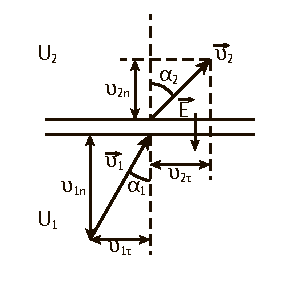
\includegraphics[width=.3\textwidth]{14_Snell} \hspace{1em}
  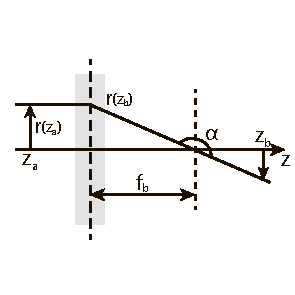
\includegraphics[width=.3\textwidth]{14_thin_lens} \hspace{1em}
  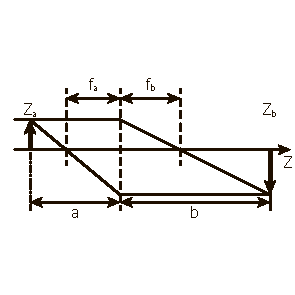
\includegraphics[width=.3\textwidth]{14_how_to_draw} \\
  \parbox{.3\textwidth}{\caption{К примеру} \label{pic14Snell}} \hspace{1em}
  \parbox{.3\textwidth}{\caption{Траектория движения заряженной частицы в
    неоднородном электростатическом поле} \label{pic14thin}} \hspace{1em}
  \parbox{.3\textwidth}{\caption{Построение изображения} \label{pic14draw}}
\end{figure}

Таким образом, в электронике аналогом коэффициента преломления является величина
\( \sqrt{U} \). Поскольку нельзя получить скачкообразное изменение потенциала,
то коэффициент преломления является некоторой функцией координат, однако
траектории электронов в неоднородном поле подобны лучам света в геометрической
оптике. Следовательно, можно создать устройства для фокусировки электронных
потоков.

\subquestion{Аналог тонкой линзы}
Проинтегрируем уравнение \eqref{eq09equation}:
\[
  \sqrt{U_0(z_b)}r'(z_b) - \sqrt{U_0(z_a)}r'(z_a) = -\frac{1}{4}
    \int\limits_{z_a}^{z_b} \frac{U_0''(z)}{\sqrt{U_0(z)}} r(z)\,dz.
\]
Здесь \( z_a \) и \( z_b \)~-- координаты в областях объекта и изображения
соответственно, штрихом обозначена производная по \( z \).

Если электрон летит параллельно оси~\( 0z \) из области объекта
(рис.~\pic{14thin}), то \( r'(z_a) = 0 \). В случае, когда область изменения
потенциала \( U_0(z) \) значительно меньше длины пролета электрона вдоль
оси~\( 0z \) (приближение тонкой линзы), можно считать, что расстояние электрона
до оси остается постоянным внутри линзы, а меняется лишь угол выхода из линзы.
Поэтому можно положить \( r(z) = r(z_a) \) и изменить пределы на бесконечные.
Тогда в плоскости выхода из линзы угол наклона электрона будет определяться
соотношением
\[
  \tg\alpha = r'(z_b) = -\frac{r(z_a)}{4\sqrt{U_0(z_b)}} \int\lii
    \frac{U_0''(z)}{\sqrt{U_0(z)}}\,dz,
\]
а фокусное расстояние:
\[
  \frac{1}{f_b} = -\frac{r'(z_b)}{r(z_a)} = \frac{1}{4\sqrt{U_0(z_b)}}
    \int\lii \frac{U_0''(z)}{\sqrt{U_0(z)}}\,dz.
\]

Повторяя те же выкладки для электрона, летящего из области изображений, получим
\[
  \frac{1}{f_a} = \frac{1}{4\sqrt{U_0(z_a)}} \int\lii
    \frac{U_0''(z)}{\sqrt{U_0(z)}}\,dz.
\]

Из последних двух уравнений следует, что
\[
  \frac{f_a}{f_b} = \sqrt{\frac{U_0(z_a)}{U_0(z_b)}}.
\]

Величины \( f_b \), \( f_a \), \( a \) и \( b \) связаны соотношением,
называемым формулой тонкой линзы:
\(
 \dfrac{f_a}{a} + \dfrac{f_b}{b} = 1
\).

\subquestion{Виды электростатических линз}

\begin{figure}[p!]
  \center
  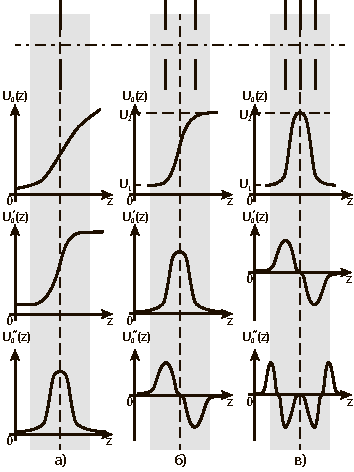
\includegraphics[width=.9\textwidth]{14_lenses} \\
  \caption{Схематическое изображение линз, распределение потенциала на оси линз,
    первых и вторых производных (затемнена область линзы): а~-- линза-диафрагма;
    б~-- иммерсионная линза; в~-- одиночная линза}
  \label{pic14lenses}
\end{figure}

На рисунке~\pic{14lenses} представлены три вида систем: линза-диафрагма~а,
иммерсионная линза~б, одиночная линза~в, графики распределения потенциалов
\( U_0(z) \), их первых \( U_0'(z) \) и вторых \( U_0''(z) \) производных.

Линза-диафрагма образуется диском с круглым отверстием, на который подается
некоторый потенциал. На рисунке приведен случай, когда \( U_0'' > 0 \)
(\( \abs{E_1} < \abs{E_2} \))~-- линза собирающая. При \( U_0'' < 0 \) линза
является рассеивающей.

Иммерсионная линза образуется двумя дисками с отверстием, на которые поданы
напряжения \( U_1 \) и \( U_2 \). Линза имеет две области: с \( U_0'' > 0 \) и
с \( U_0'' < 0 \). В первой области пучок фокусируется, во второй~--
расфокусируется, но так как скорость электронов во второй области больше, чем в
первой, то электроны пролетают расфокусирующий участок быстрее, чем
фокусирующий. Вследствие этого общее действие линзы всегда является собирающим.

Одиночная линза состоит из трех электродов. На крайние подается одинаковый
потенциал, а на средний~-- иной. Здесь имеется две собирающие области и одна
рассеивающая. По аналогичному с иммерсионной линзой принципу эта линза является
фокусирующей.
